\documentclass[12pt]{article}
\usepackage[]{fullpage}
%\usepackage{a4wide}
\usepackage[]{graphics}
\usepackage{natbib}
\usepackage{setspace} 
\usepackage{url}
\usepackage{amsmath}
\usepackage{mathtools}


\title{Supervised and Unsupervised Learning on Lending Club Data}
\author{Muhammad Waqar Ayub Khan, UEA ID. 100334069}

\begin{document}

\maketitle

\begin{abstract}
	
\onehalfspacing

Classification and clustering are difficult tasks that can be used to predict results from various datasets. These are the tasks that make up the majority of data science work. On the lending club dataset, this study uses various KDD actions for classification and clustering, which enable the related institute to identifying whether a loan is potentially a bad loan or a good loan. To obtain reliable results, various machine learning algorithms for classification and clustering were applied to the dataset.

\end{abstract}
\doublespacing

\section{Introduction}
This report has two task, first task is to use lending club dataset and predict the loan status of the accounts, as we already know the loan status so this can be done by using different classification algorithms and then we can find the accuracy of our predictions by comparing the predicted results with the actual loan status. Second task is to use clustering algorithms to divide the data points into number of groups, each group represents the similar type of data points in our case loan status. Both tasks consists on Knowledge Discovery of Databases (KDD) steps, each step of KDD has a separate action on dataset which helps in getting more accurate results. In this study various techniques was used on dataset before making predictions such as removing abnormal data points known as Outliers, dealing with missing values, data balancing, dimensionality reduction which are the part of KDD process. Classification and clustering both involves these steps for accurate predictions, these steps are known as Cleaning and Pre-processing of a data. After getting cleaned and pre-processed data, for classification various algorithms were applied to get predictions and similarly for clustering predictions different clustering algorithms were applied to get accurate clusters. Overall both classification and clustering involve cleaning, pre-processing, modeling, evaluation, each step for both clustering and classification will be discussed in this report.

\section{Data / Feature Summary} 
Lending club data contains 108 different columns and have 77159 different loan account records. Out of 108 there 17 columns have more than 60 percent null values, having more much null values might lead to bad prediction so these features were dropped from the dataset and new dataset was created which has 91 columns or features with same number of rows. Figure \ref{fig:MissingValues} shows the feature having missing values greater than 60 percent.
\begin{figure}[h!]
	\centering
	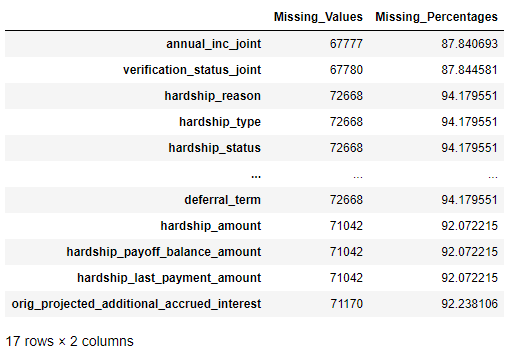
\includegraphics{MissingValues.png}
	\caption{Features having more than 6 percent missing values}
	\label{fig:MissingValues}
\end{figure}
After dropping these features we have a data with 91 features out of 91 14 features are categorical, which are shown in table \ref{table:1}.
\begin{table}[h!]
	\centering
	\begin{tabular}{ |p{3cm}|p{3cm}|p{3cm}|  }
		\hline
		\multicolumn{2}{|c|}{Categorical Features} \\

		\hline
		$emp\_title$ & 28185 \\
		$home\_ownership$ & 5 \\
		$loan\_status$ & 7 \\
		$int\_rate$ & 129 \\
		$term$ & 2 \\
		$grade$ & 7 \\
		$earliest\_cr\_line$ & 622 \\
		$issue\_d$ & 16 \\
		$last\_pymnt\_d	$ & 28 \\
		$next\_pymnt\_d	$ & 9 \\
		$verification\_status$ & 3 \\
		$pymnt\_plan$ & 1 \\
		$purpose$ & 13 \\
		$revol\_util$ & 1074 \\
		\hline
	\end{tabular}
	\caption{List of Categorical Features with unique values}
	\label{table:1}
\end{table}
 Features named such as id, $emp\_title$ will be dropped because these two has too many unique values, $pymnt\_plan$ will also be dropped because it has only one unique value. $int\_rate$ and $revol\_util$ will be converted to numeric after removing $\%$ symbol from the last similarly $term$ will be converted to numeric after removing $months$ from last. There are some dates columns or features in the data we can use these dates and can convert those dates into some useful information like missing term or remaining term. Figure \ref{fig:dates} shows the features which have been transformed from the dates columns. $loan\_status$ is a target feature which will be separated from the other columns or features. The remaining categorical features or columns will now be encoded into the numeric so that these features can be dealt by modeling algorithms. These are encoded before the train-test split because encoding before split reduce the computation and does not expose the test data to the training model. After feature engineering, encoding the new data has only one categorical feature which is $loan\_status$ and it will be remove from data as it is target feature and new data has now 85 columns or features and 77159 records.

\begin{figure}[h!]
	\centering
	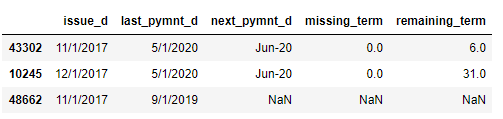
\includegraphics{dates.png}
	\caption{Transformation of Dates Columns}
	\label{fig:dates}
\end{figure}

\section{Methods used for Ensemble Learning}

\subsection{Boosting}
According to \citep{freund1996experiments} and \citep{zhou2012ensemble}, in boosting, a series of algorithms is used to transform poor learners to strong learners, as the weak learner performs better than a random assumption, and the strong learner performs near to ideal overall output. \citep{zhou2012ensemble} describes the boosting with a simple example which is as follows: Consider we have got dataset X which is composed of $x_1$, $x_2$, $x_3$ each take $1/3$ distribution space, and we have got a learner operating in random guess has the 50\% errors rate. We want to get more accurate results, but after applying weak learners we only manage to get the correct result in $x_1$ and $x_2$ and has a $1/3$ error rate and let us say the result of this classifier is $h_1$. Boosting works through enhancing the mistakes of preceding learners results in our case, it is $h_1$. Now we must distribute a new space $d'$ from $d$. In this new space, the learner will give more attention to $x_3$ as it was categorized incorrectly in the first strive at the same time as producing $h_2$. The $h_2$ correctly classify the $x_1$ and $x_3$ and incorrectly classify the $x_2$. So the combined classifier will successfully classify the $x_1$ and bring mistakes for the $x_2$ and $x_3$. Again we calculate new space from $d'$ to $d''$ and bypass this $d''$ space to the learner which generates $h_3$ so $h_3$ correctly classifies the $x_2$ and $x_3$ and incorrectly classifies the $x_1$. Now by way of combining $h_1$, $h_2$, and $h_3$ we have got a more accurate combined classifier, in view that in each space at least two classifiers make accurate predictions. Figure \ref{fig:GeneralBoosting} taken from \citep{zhou2012ensemble} gives the general idea of boosting. 
               \begin{figure}[h!]
               	\centering
               	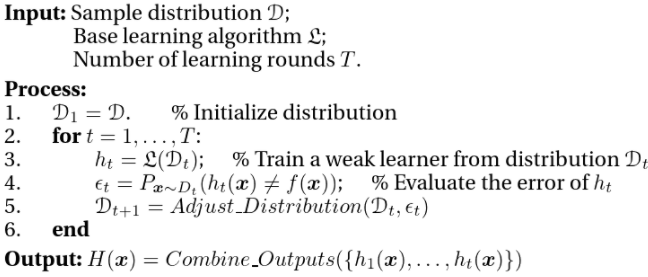
\includegraphics{GeneralBoosting.png}
               	\caption{General Boosting Flow ~\citep{zhou2012ensemble}}
               	\label{fig:GeneralBoosting}
               \end{figure}
               In general boosting explanation, the space transformation (Calculating the dataset for next leaner), and combining methods are not described clearly. The new boosting technique by \citep{freund1996experiments} has stated these two elements in-depth and that method is referred to as Adaboost.
               
               
{\bf{Adaboost}}

\citep{freund1996experiments} expressed that Adaboost accepts input of training dataset which can be of m length such as:
	\begin{align*}
		S = ((x_1, y_1), (x_2, y_2) ….. (x_m, y_m) ~\citep{freund1996experiments}
	\end{align*}

Where the $x_i$ = set of features in the training dataset and $y_i$ = class labels and pass this dataset to the weak learners of the ensemble which will give $h_t$: $X\,\to\,Y$, where $h_t$ = the hypothesis of the weak learner, this hypothesis should be with the minimum error i-e \\ $(\epsilon_t = Pr_{i \sim D_t}[h_t(x_i)\neq  y_i])~\citep{freund1996experiments}$. This process will be repeated till T times on each iteration error will be calculated and a new dataset for the next round will be generated. Figure \ref{fig:Adaboost} shows the algorithm for the AdaBoost which is taken from \citep{freund1996experiments}. 
\begin{figure}[h!]
	\centering
	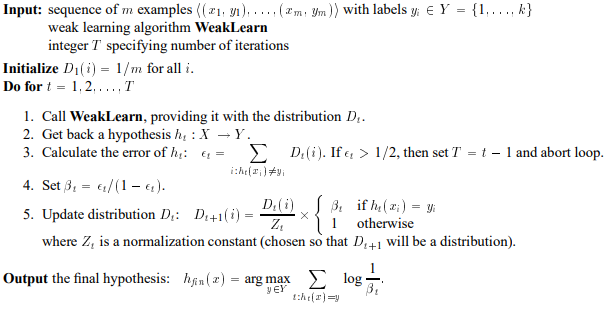
\includegraphics{Adaboost.png}
	\caption{Adaboost Algoritm ~\citep{freund1996experiments}}
	\label{fig:Adaboost}
\end{figure}
In figure \ref{fig:Adaboost} two unspecified concepts can be seen(1) how $D_t$ is computed (2) how $h_fin$ is computed. Every boosting technique has its way to tackle these concepts. There are various versions of Adaboost, yet in this report Adaboost.M1 and Adaboost.M2 will be examined. In Adaboost.M1 the initial distribution $D_i$ is set to $1/m$ and $D_{i+1}$ is calculated from $D_i$. For $D_{i+1}$ we have to multiply the weight of $i$ with $ \beta_t $(Which is shown in figure \ref{fig:Adaboost}) if $h_t$ classifies $x_i$ correctly else weight remains the same. The weights are renormalized by dividing with Z$_t$(Normalization Constant). In short in Adaboost $x_i$ which is incorrectly classified in the previous classier will gain weight and $x_i$ which are classified correctly in the previous classifier will lose weight because of this in the next classifier there are chances $x_i$ which was incorrectly classified will be selected as the dataset for the next weak learner. Note that classifier and weak learners are the same. 
\citep{freund1996experiments} expressed that the fundamental inconvenience of Adaboost.M1 is that it does not manage the weak learners with an error of more than $1/2$, the expected error weak learner can get is $1 - 1/k$ (the $k$= number of class marks), however, when $k > 2$ it is not possible to get an error less than $1/2$. We can say that Adaboost.M1 is useful for binary classification problems, however, for multiple classifications we need to discover some new strategies. Adaboost.M2 overcome this problem by communicating with boosting algorithm and learning algorithm. We expect that weak learners provide more descriptive results rather than identifying a single result.
 \citep{freund1996experiments} gave the example of OCR(Optical character recognition) it may be hard to tell the character is 7 or 9 our weak learner may output \{7, 9\}. In Adaboost.M2 we interpret the $h_t$ in a binary form. The weak hypothesis can be concluded in the following way. If $h_t(x_i, y_i) = 1$ and $h_t(x_i, y)=0$, then $h_t$ is correctly classified that $x_i's$ label is $y_i's$ not $y$ on the other hand, if $h_t(x_i, y_i) = 0$ and $h_t(x_i, y)=1$ then $h_t$ has classified the result incorrectly and if $h_t(x_i, y)=h_t(x_i, y_i)$ then $h_t$ will be considered as a random guess. In Adaboost.M2 instead of dealing with error, there is a pseudo-loss which can be calculated using the expression shown in figure \ref{fig:pseudoLoss}. 
 \begin{figure}[h!]
 	\centering
 	\includegraphics{pseudoLoss.png}
 	\caption{Adaboost.M2 Pseudo-Loss ~ \citep{freund1996experiments}}
 	\label{fig:pseudoLoss}
 \end{figure}
 So the goal of the weak learner in Adaboost.M2 is to produce $h_t$ with less pseudo-loss. In Adaboost.M2 weak learners have pseudo-loss slightly better than ½ regardless of the number of classes so which means Adaboost.M2 can handle the multi-classification problem.
 
 
\citep{freund1996experiments} address that boosting may be useful if the problem has two of the following properties. The first property is that training data need to have various degrees of hardness. Indirectly training the weak algorithms in such a way that they deal with a harder set of training data. The second property is that the weak learner is adaptable to adjustments within the learning dataset also known as “Unstable Behavior” of the training dataset.

\subsection{Bagging}
\citep{huang2009research} depicts that bagging is an ensemble approach that trains the number of weak learners, each with a distinct bootstrap sample. The bootstrap sample is received through a subsampling of training dataset with replacement. Training the weak learner with a distinctive sample set will increase the diversity of the ensemble learner which increases the accuracy of the ensemble learner. The algorithm taken from \citep{huang2009research} is shown in figure \ref{fig:bagging}. 
 \begin{figure}[h!]
 	\centering
	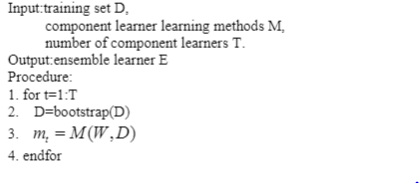
\includegraphics{bagging.png}
	\caption{Bagging ~\citep{huang2009research}}
	\label{fig:bagging}
\end{figure}
\citep{breiman1996bagging} explains bagging mathematically that the learning set of $\pounds$ includes data $\{(y_n, x_n), n=1….N\}$ where $x_n$ is the set of attribute and $y_n$ is the predicted class label or numerical value. Assume we have method $\phi (x, \pounds)$ that operates as a predictor. If $x$ is the input we can predict $y$ by using $\phi (x, \pounds)$ that’s the traditional machine learning approach. Now think we have $\{L_k\}$: the sequence of learning sets each includes N independent observations, so by using of $\{L_k\}$ we have to find a better predictor than the single weak predictor. If y is a numerical value, the average of $\phi (x, \pounds)$ is used instead of $\phi (x, \pounds)$, and if it is a class label, a voting technique among weak learners is used. This average and vote casting approach is referred to as aggregation. Distribution of learning set $\pounds$ over the weak learners is referred to as bootstrapping. Breman called this entire method “Bootstrap aggregation” and use the acronym bagging. Like boosting bagging is also adaptive to the unexpected adjustments that may arise in learning $\pounds$. \citep{breiman1996bagging} performs some experiments in which he examines the error rates of different datasets calculated using 10-fold cross validation and bootstrap sampling, he determined that error rates with bootstrap sampling (Bagging) are improved as compare to 10-fold cross-validation. He executed bagging classification and bagging regression in both the scenarios bagging had improved error rates. Figure \ref{fig:baggingResults} taken from \citep{breiman1996bagging} indicates the results of the experiments.
 \begin{figure}[h!]
 	\centering
	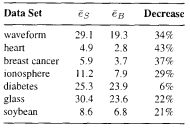
\includegraphics{baggingClassification.png}
	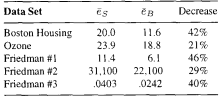
\includegraphics{baggingRegression.png}
	\caption{\citep{breiman1996bagging} Classification and Regression Results}
	\label{fig:baggingResults}
\end{figure}

\subsection{Stacking}
The idea well explained in \citep{zhou2012ensemble} is that stacking is a manner in which a combining learner called the second-level learner is taught to integrate the outcomes of the individual learners called the first-level learner. The idea is to use training data to train the first-level learners and then create a new dataset for the second-level learners. The output of the first-level learner along with the actual class labels is the input of the second-level learner. Stack ensembles are specifically heterogeneous because the first-level learners are trained via a distinctive set of algorithms, however, they might be homogeneous. Figure \ref{fig:stacking} from \citep{zhou2012ensemble} shows the pseudo-code for the stacking. 
 \begin{figure}[h!]
 	\centering
	\includegraphics{stacking.png}
	\caption{Stacking Pseudo-Code ~\citep{zhou2012ensemble}}
	\label{fig:stacking}
\end{figure}
One important factor raised by \citep{zhou2012ensemble} is that if the same data used for extracting the dataset for the second-level learner that turned into used for the training of the first-level learner then there might be the chance of overfitting so it is important to keep data for extracting new datasets for second-level learners separated from training data. Cross-validation is often encouraged. \citep{zhou2012ensemble} said assume D: Training dataset cut up into randomly k equal parts $D_1,….., D_k$ and $D_j or D(-j) = D / D(j)$ to be the testing and training dataset for the $j^{th}$ fold. T is the set of learning algorithms, $h_t(-j)$ is the learner of $t^{th}$ learner algorithm on $D(-j)$. For each $x_i$ (test set in the $j^{th}$ fold) $z_it$ is the output of the learner $h_t(-j)$ on $x_i$ so after all the $j^{th}$ iterations the brand new dataset from T learners is as follows: $D' = \{(z_i1,....,z_iT), y_i\}^{m}_{i=1}$.

The above dataset is then handed to the second-level learner and final $h'$ can be acquired as: $( z_1 , . . . , z_T )$


\section{Issues related to ensemble learning}
A lot of research was performed on ensemble learning in the past still, there are a few problems related to ensemble learning that needs consideration. \citep{wang2008some} said that among all the issues, factors that effecting the accuracy of an ensemble is the important one because everyone is concern about the accurate outcomes. As in keeping with \citep{wang2008some}, the factors that outcomes the accuracy of the ensemble are D: diversity among member models, acc(mi): the accuracy of the individual model, N: the number of member models, and S: decision-making strategy. These elements can be denoted as:
$acc(V) = f ( acc(m_i) \forall_i = 1toN,D,S,N) ~\citep{wang2008some}$.
According to \citep{wang2008some} while analyzing unique single factors, other factors cannot be sidelined because these factors are exceedingly correlated with each other. The focus of the \citep{wang2008some} is the experiment that was performed on different sets of data to explain the brief concept of how the above factors are related to each other and the way they impact the accuracy of the ensemble. Figure \ref{fig:issues} indicates the test results of \citep{wang2008some}. 
 \begin{figure}[h!]
 	\centering
	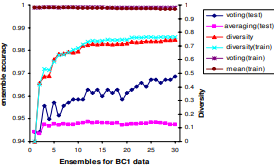
\includegraphics{issues.png}
	\caption{Factors effecting the accuracy ~\citep{wang2008some}}
	\label{fig:issues}
\end{figure}
Figure \ref{fig:issues} depicts that there may be nearly no diversity when the number of models is very fewer (N$\textless$3), after that when the number of model increases diversity also increases. After certain limit diversity still increases, but at a very low rate. The increase in diversity will lead to an increase in ensemble accuracy.
From figure \ref{fig:issues} it can be seen that ensemble accuracy stays consistent when using the average decision-making strategy which depicts that if the average strategy is used to get ensemble accuracy diversity does not create an effect on the results. On the opposite hand, while the vote casting strategy is used the continuous increase in ensemble accuracy can be seen as diversity of the ensemble increases. The closing ten models used in the ensemble are selection trees that play very awful individually, but after adding to the ensemble, increases in diversity occurs consequently accuracy of the ensemble will increase which concludes that much less accurate individual models will increase the diversity of the ensemble which ultimately increases the accuracy of the ensemble. From figure \ref{fig:issues} it could be depicted that after the increase in the number of models the diversity of an ensemble increases which indirectly leads to the increase in accuracy of an ensemble. In figure \ref{fig:issues} a thrilling factor is discovered that there is up-down instability may be visible. This is due to the fact when even number of models are located the win-threshold for the voting strategy increases, but when the number of the models will increase this difference becomes smaller and can be negligible. This point concludes that why the odd number of models ought to be selected because if the win-threshold value is lower ensemble provides more correct results in voting strategy.

\section{Conclusion}
This report has covered a few foundations of ensemble which were set in 1990's, after knowing some foundation this report depicted the ensemble learning in detail i-e combining the distinctive individual model with diverse data so the precise outcomes of the ensemble can be accomplished. Reasons of ensembles performing better compared to the individual model are additionally notice in the report among every one of the reasons the most significant is that ensemble learning because of its diversity eliminate overfitting from the model which prompts low variance and low bias which indirectly improve results. Some popular ensemble learning techniques are likewise discussed in this report are bagging, boosting, stacking. Bagging was presented in \citep{breiman1996bagging} which dependent on the idea of bootstrapping and aggregation, detailed working of bagging is well explained in this report. The second technique which examined is boosting which depends on the idea of lifting the weights of incorrect classified results so that they can be selected as a dataset for the next learner, detail along with different versions of boosting is discussed in the report. The last technique for ensemble is stacking which uses a learning algorithm for combining results as opposed to casting a vote and averaging considered as the second-level learner and individual learners that produces results called the first-level learner. In the absolute last a test result has been analyzed which shows what various factors can be meant for the precision of the ensemble, diversity assumes a significant part as the diversity of an ensemble increases the accuracy of an ensemble increases. This report covers the total image of ensemble learning, strategies used for ensemble, and factors that can impact the exactness of the ensemble.

\singlespacing

\bibliographystyle{agsm}
\bibliography{document}

\end{document}




